\documentclass[aspectratio=43]{beamer}

\usetheme{Boadilla}
\setbeamertemplate{footline}[page number]{}
\setbeamertemplate{navigation symbols}{}

\usepackage{times}
\usepackage{tikz}
\usefonttheme{structurebold}
\usepackage{listings}

% Suppress the navigation bar
\beamertemplatenavigationsymbolsempty

\newenvironment{changemargin}[1]{% 
  \begin{list}{}{% 
    \setlength{\topsep}{0pt}% 
    \setlength{\leftmargin}{#1}% 
    \setlength{\rightmargin}{1em}
    \setlength{\listparindent}{\parindent}% 
    \setlength{\itemindent}{\parindent}% 
    \setlength{\parsep}{\parskip}% 
  }% 
  \item[]}{\end{list}} 

\title{Lecture 03---Gustafson's Law, Concurrency~vs~Parallelism}
\subtitle{ECE 459: Programming for Performance}
\author{Patrick Lam}
\institute{University of Waterloo}
\date{January 9, 2015}

\begin{document}

%%%%%%%%%%%%%%%%%%%%%%%%%%%%%%%%%%%%%%%%%%%%%%%%%%%%%%%%%%%%%%%%%%%%%%%%%%%%%%%%
\begin{frame}[plain]
  \titlepage
\end{frame}
%%%%%%%%%%%%%%%%%%%%%%%%%%%%%%%%%%%%%%%%%%%%%%%%%%%%%%%%%%%%%%%%%%%%%%%%%%%%%%%%

\part{Limitations to Parallelism}

%%%%%%%%%%%%%%%%%%%%%%%%%%%%%%%%%%%%%%%%%%%%%%%%%%%%%%%%%%%%%%%%%%%%%%%%%%%%%%%%
\begin{frame}
  \frametitle{Multiprocessing in Three Acts}

  \begin{changemargin}{2cm}
    Act 1: {\bf Attack of the Clones}\\
    \hspace*{1em} (symmetric multiprocessing systems) \\[1em]
    Act 2: {\bf The Empire Strikes Back}\\
    \hspace*{1em} (Amdahl's Law) \\[1em]
    Act 3: {\bf A New Hope}\\
    \hspace*{1em} (Gustafson's Law)
  \end{changemargin}
\end{frame}
%%%%%%%%%%%%%%%%%%%%%%%%%%%%%%%%%%%%%%%%%%%%%%%%%%%%%%%%%%%%%%%%%%%%%%%%%%%%%%%%

\section{Amdahl's Law: Wrap-up}
%%%%%%%%%%%%%%%%%%%%%%%%%%%%%%%%%%%%%%%%%%%%%%%%%%%%%%%%%%%%%%%%%%%%%%%%%%%%%%%%
\begin{frame}
  \frametitle{Amdahl's Law Generalization}

  \hspace*{2em} \begin{minipage}{.8\textwidth} The program may have many parts, each of which we can tune to
  a different degree.\\[1em]

  Let's generalize Amdahl's Law.\\[1em]

  $f_1, f_2, \ldots, f_n$: fraction of time in part $n$

  $S_{f_1}, S_{f_n}, \ldots, S_{f_n}$: speedup for part $n$
\end{minipage}
  \vfill
  \begin{center}
  \structure{\[\mbox{\em speedup} = \frac{1}{\frac{f_1}{S_{f_1}} + \frac{f_2}{S_{f_2}} + \ldots +
    \frac{f_n}{S_{f_n}}}\]}
  \end{center}
\end{frame}
%%%%%%%%%%%%%%%%%%%%%%%%%%%%%%%%%%%%%%%%%%%%%%%%%%%%%%%%%%%%%%%%%%%%%%%%%%%%%%%%

%%%%%%%%%%%%%%%%%%%%%%%%%%%%%%%%%%%%%%%%%%%%%%%%%%%%%%%%%%%%%%%%%%%%%%%%%%%%%%%%
\begin{frame}
  \frametitle{Application (1)}

  \hspace*{2em} 
  \begin{minipage}{.8\textwidth} Consider a program with 4 parts in the following scenario:\\[2em]
    \begin{tabular}{r|r|r|r}
    \multicolumn{2}{l}{} & \multicolumn{2}{c}{Speedup} \\
    Part & Fraction of Runtime & Option 1 & Option 2\\
    \hline
    1 & 0.55 & 1  & 2\\
    2 & 0.25 & 5  & 1\\
    3 & 0.15 & 3  & 1\\
    4 & 0.05  & 10 & 1\\
  \end{tabular}

~\\[2em]
  We can implement either Option 1 or Option 2. \\
  Which option is better?
  \end{minipage}
\end{frame}
%%%%%%%%%%%%%%%%%%%%%%%%%%%%%%%%%%%%%%%%%%%%%%%%%%%%%%%%%%%%%%%%%%%%%%%%%%%%%%%%

%%%%%%%%%%%%%%%%%%%%%%%%%%%%%%%%%%%%%%%%%%%%%%%%%%%%%%%%%%%%%%%%%%%%%%%%%%%%%%%%
\begin{frame}
  \frametitle{Application (2)}

\begin{minipage}{.8\textwidth}
  \hspace*{2em} ``Plug and chug'' the numbers:\\[1em]
\hspace*{.2\textwidth}\begin{minipage}{.8\textwidth}
  {\bf Option 1} \vspace*{-2em}

  \[ \mbox{\em speedup} = \frac{1}{0.55 + \frac{0.25}{5} + \frac{0.15}{3} + \frac{0.05}{5}}
    = 1.53  \]
~\\[1em]
  {\bf Option 2} \vspace*{-2em}

   \[\mbox{\em speedup} = \frac{1}{\frac{0.55}{2} + 0.45} = 1.38 \hspace*{5.5em}\]
\end{minipage}
\end{minipage}

\end{frame}
%%%%%%%%%%%%%%%%%%%%%%%%%%%%%%%%%%%%%%%%%%%%%%%%%%%%%%%%%%%%%%%%%%%%%%%%%%%%%%%%

%%%%%%%%%%%%%%%%%%%%%%%%%%%%%%%%%%%%%%%%%%%%%%%%%%%%%%%%%%%%%%%%%%%%%%%%%%%%%%%%
\begin{frame}
  \frametitle{Empirically estimating parallel speedup P}

  \hspace*{2em} Useful to know, don't have to commit to memory:
  \vfill
  \[P_{\mbox{\scriptsize estimated}} = \frac{\frac{1}{\mbox{\em speedup}}-1}{\frac{1}{N}-1}\]
  \vfill
  \hspace*{2em} \begin{minipage}{.8\textwidth} \begin{itemize}
    \item Quick way to guess the fraction of parallel code
    \item Use $P_{\mbox{\scriptsize estimated}}$ to predict speedup for a different number of processors
  \end{itemize} \end{minipage}
\end{frame}
%%%%%%%%%%%%%%%%%%%%%%%%%%%%%%%%%%%%%%%%%%%%%%%%%%%%%%%%%%%%%%%%%%%%%%%%%%%%%%%%

%%%%%%%%%%%%%%%%%%%%%%%%%%%%%%%%%%%%%%%%%%%%%%%%%%%%%%%%%%%%%%%%%%%%%%%%%%%%%%%%
\begin{frame}
  \frametitle{Summary of Amdahl's Law}

\hspace*{2em} Important to focus on the part of the program with most impact.\\[1em]

\hspace*{2em} Amdahl's Law:\\[1em]
\hspace*{2em} \begin{minipage}{.8\textwidth}
  \begin{itemize}
    \item estimates perfect performance gains from
          parallelization (under assumptions); but,
    \vfill
    \item only applies to solving a \structure{fixed problem size} in the
          shortest possible period of time
  \end{itemize} \end{minipage}
\end{frame}
%%%%%%%%%%%%%%%%%%%%%%%%%%%%%%%%%%%%%%%%%%%%%%%%%%%%%%%%%%%%%%%%%%%%%%%%%%%%%%%%


\section{Gustafson's Law}
%%%%%%%%%%%%%%%%%%%%%%%%%%%%%%%%%%%%%%%%%%%%%%%%%%%%%%%%%%%%%%%%%%%%%%%%%%%%%%%%
\begin{frame}
  \frametitle{Gustafson's Law: Formulation}

\hspace*{2em} \begin{minipage}{.8\textwidth}
\begin{tabbing}
  $n$:~~~~~~ \= problem size\\[.1em]

  $S(n)$: \> fraction of serial runtime for a parallel execution\\[.1em]

  $P(n)$: \> fraction of parallel runtime for a parallel execution\\
\end{tabbing}
\end{minipage}

\begin{eqnarray*}
T_p &=& S(n) + P(n) = 1 \\
T_s &=& S(n) + N \cdot P(n) 
\end{eqnarray*}

\[ \mbox{\em speedup} = \frac{T_s}{T_p} \]
\end{frame}
%%%%%%%%%%%%%%%%%%%%%%%%%%%%%%%%%%%%%%%%%%%%%%%%%%%%%%%%%%%%%%%%%%%%%%%%%%%%%%%%

%%%%%%%%%%%%%%%%%%%%%%%%%%%%%%%%%%%%%%%%%%%%%%%%%%%%%%%%%%%%%%%%%%%%%%%%%%%%%%%%
\begin{frame}
  \frametitle{Gustafson's Law}

\hspace*{2em}\begin{minipage}{.8\textwidth}
  \structure{$speedup = S(n) + N \cdot P(n)$}\\[1em]

  Assuming the fraction of runtime in serial part decreases as $n$ increases,
  the speedup approaches $N$.

  \begin{itemize}
    \item Yes! Large problems can be efficiently parallelized. (Ask Google.)
  \end {itemize}
\end{minipage}
\end{frame}
%%%%%%%%%%%%%%%%%%%%%%%%%%%%%%%%%%%%%%%%%%%%%%%%%%%%%%%%%%%%%%%%%%%%%%%%%%%%%%%%

\section{}
%%%%%%%%%%%%%%%%%%%%%%%%%%%%%%%%%%%%%%%%%%%%%%%%%%%%%%%%%%%%%%%%%%%%%%%%%%%%%%%%
\begin{frame}
  \frametitle{Driving Metaphor}

  {\bf Amdahl's Law}
  
  Suppose you're travelling between 2 cities 90~km apart. If you travel for an
  hour at a constant speed less than 90 km/h, your average will never equal
  90~km/h, even if you energize after that hour.
  \vfill
  {\bf Gustafson's Law}

  Suppose you've been travelling at a constant speed less than 90~km/h. Given
  enough distance, you can bring your average up to 90~km/h.
\end{frame}
%%%%%%%%%%%%%%%%%%%%%%%%%%%%%%%%%%%%%%%%%%%%%%%%%%%%%%%%%%%%%%%%%%%%%%%%%%%%%%%%


\part{Parallelism versus Concurrency}
\begin{frame}
 
  \partpage
\end{frame}

%%%%%%%%%%%%%%%%%%%%%%%%%%%%%%%%%%%%%%%%%%%%%%%%%%%%%%%%%%%%%%%%%%%%%%%%%%%%%%%%
\begin{frame}
  \frametitle{Parallelism versus Concurrency}

\begin{changemargin}{2cm}
  {\bf Parallelism}

  Two or more tasks are \structure{parallel}\\ \hspace*{2em} if they are running at the same time. 

  Main goal: run tasks as fast as possible. 

  Main concern: \structure{dependencies}.
  \vfill
  {\bf Concurrency}

  Two or more tasks are \structure{concurrent}\\ \hspace*{2em} if the ordering of the two tasks is not 
  predetermined. 

  Main concern: \structure{synchronization}.
\end{changemargin}

\end{frame}
%%%%%%%%%%%%%%%%%%%%%%%%%%%%%%%%%%%%%%%%%%%%%%%%%%%%%%%%%%%%%%%%%%%%%%%%%%%%%%%%

\part{Threads}
\begin{frame}
  \partpage
\end{frame}
%%%%%%%%%%%%%%%%%%%%%%%%%%%%%%%%%%%%%%%%%%%%%%%%%%%%%%%%%%%%%%%%%%%%%%%%%%%%%%%%
\begin{frame}
  \frametitle{Threads}

  \begin{center}
    \includegraphics[scale=0.1]{L03/thread}
  \end{center}

  \begin{changemargin}{2.5cm}
  \begin{itemize}
    \item What are they?
    \vfill
    \item How do operating systems implement them?
    \vfill
    \item How can we leverage them?
  \end{itemize}
  \end{changemargin}
\end{frame}
%%%%%%%%%%%%%%%%%%%%%%%%%%%%%%%%%%%%%%%%%%%%%%%%%%%%%%%%%%%%%%%%%%%%%%%%%%%%%%%%

%%%%%%%%%%%%%%%%%%%%%%%%%%%%%%%%%%%%%%%%%%%%%%%%%%%%%%%%%%%%%%%%%%%%%%%%%%%%%%%%
\begin{frame}
  \frametitle{Processes versus Threads}

\begin{changemargin}{2.5cm}
  {\bf Process}

  An instance of a computer program that contains program code and its:

  \begin{itemize}
    \item Own address space / virtual memory;
    \item Own stack / registers;
    \item Own resources (file handles, etc.).
  \end{itemize}
  \vfill
  {\bf Thread}

  ``Lightweight processes''. 

  In most cases, a thread is contained within a process.

  \begin{itemize}
    \item Same address space as parent process
      \begin{itemize}
        \item Shares access to code and variables with parent.
      \end{itemize}
    \item Own stack / registers
    \item Own thread-specific data
  \end{itemize}

\end{changemargin}

\end{frame}
%%%%%%%%%%%%%%%%%%%%%%%%%%%%%%%%%%%%%%%%%%%%%%%%%%%%%%%%%%%%%%%%%%%%%%%%%%%%%%%%

%%%%%%%%%%%%%%%%%%%%%%%%%%%%%%%%%%%%%%%%%%%%%%%%%%%%%%%%%%%%%%%%%%%%%%%%%%%%%%%%
\begin{frame}
  \frametitle{Software and Hardware Threads}

\begin{changemargin}{2.5cm}
  {\bf Software Thread:}

  What you program with (e.g. with {\tt pthread\_create()} or {\tt std::thread()}). \vfill

  Corresponds to a stream of instructions executed by the processor. \vfill

  On a single-core, single-processor machine, someone has to multiplex the CPU to
  execute multiple threads concurrently; only one thread runs at a time.

  \vfill
  {\bf Hardware Thread:}

  Corresponds to virtual (or real) CPUs in a system. Also known as strands. \vfill

  Operating system must multiplex software threads onto hardware threads, but 
  can execute more than one software thread at once.

\end{changemargin}

\end{frame}
%%%%%%%%%%%%%%%%%%%%%%%%%%%%%%%%%%%%%%%%%%%%%%%%%%%%%%%%%%%%%%%%%%%%%%%%%%%%%%%%


%%%%%%%%%%%%%%%%%%%%%%%%%%%%%%%%%%%%%%%%%%%%%%%%%%%%%%%%%%%%%%%%%%%%%%%%%%%%%%%%
\begin{frame}
  \frametitle{Thread Model---1:1 (Kernel-level Threading)}

    \begin{changemargin}{1.5cm}

    Simplest possible threading implementation.
    \vfill
    The kernel schedules threads on different processors;
      \begin{itemize}
        \item NB: Kernel involvement required to take advantage of a multicore system.
      \end{itemize}
    \vfill
    Context switching involves system call overhead.
    \vfill
    Used by Win32, POSIX threads for Windows and Linux.
    \vfill
    Allows concurrency and parallelism.

    \end{changemargin}
\end{frame}
%%%%%%%%%%%%%%%%%%%%%%%%%%%%%%%%%%%%%%%%%%%%%%%%%%%%%%%%%%%%%%%%%%%%%%%%%%%%%%%%

%%%%%%%%%%%%%%%%%%%%%%%%%%%%%%%%%%%%%%%%%%%%%%%%%%%%%%%%%%%%%%%%%%%%%%%%%%%%%%%%
\begin{frame}
  \frametitle{Thread Model---N:1 (User-level Threading)}

  \begin{changemargin}{1.5cm}
    All application threads map to a single kernel thread.
    \vfill
    Quick context switches, no need for system call.
    \vfill
    Cannot use multiple processors, only for concurrency.
      \begin{itemize}
        \item Why would you use user threads?
      \end{itemize}
    \vfill
    Used by GNU Portable Threads.
  \end{changemargin}
\end{frame}
%%%%%%%%%%%%%%%%%%%%%%%%%%%%%%%%%%%%%%%%%%%%%%%%%%%%%%%%%%%%%%%%%%%%%%%%%%%%%%%%

%%%%%%%%%%%%%%%%%%%%%%%%%%%%%%%%%%%%%%%%%%%%%%%%%%%%%%%%%%%%%%%%%%%%%%%%%%%%%%%%
\begin{frame}
  \frametitle{Thread Model---M:N (Hybrid Threading)}

  \begin{changemargin}{1.5cm}
    Map $M$ application threads to $N$ kernel threads.
    \vfill
    A compromise between the previous two models.
    \vfill
    Allows quick context switches and the use of multiple processors.
    \vfill
    Requires increased complexity:
    \begin{itemize}
        \item Both library and kernel must schedule.
        \item Schedulers may not coordinate well together.
        \item Increases likelihood of priority inversion\\ \hspace*{2em} (recall from Operating Systems).
      \end{itemize}
    \vfill
    Used by Windows 7 threads.
  \end{changemargin}
\end{frame}
%%%%%%%%%%%%%%%%%%%%%%%%%%%%%%%%%%%%%%%%%%%%%%%%%%%%%%%%%%%%%%%%%%%%%%%%%%%%%%%%

%%%%%%%%%%%%%%%%%%%%%%%%%%%%%%%%%%%%%%%%%%%%%%%%%%%%%%%%%%%%%%%%%%%%%%%%%%%%%%%%
\begin{frame}
  \frametitle{Live Coding Demo: Deducing the Thread Model}

  \begin{changemargin}{2cm}
    {\tt time}, {\tt top}, and {\tt perf stat} all let you figure this out.
  \end{changemargin}

\end{frame}
%%%%%%%%%%%%%%%%%%%%%%%%%%%%%%%%%%%%%%%%%%%%%%%%%%%%%%%%%%%%%%%%%%%%%%%%%%%%%%%%

\part{Types of Multiprocessing}
\begin{frame}
  \partpage
\end{frame}

%%%%%%%%%%%%%%%%%%%%%%%%%%%%%%%%%%%%%%%%%%%%%%%%%%%%%%%%%%%%%%%%%%%%%%%%%%%%%%%%
\begin{frame}[fragile]
  \frametitle{Example System---Physical View}
  
  \begin{center}
  \includegraphics[scale=0.25]{L03/computer-parts}
  \end{center}

  \begin{itemize}
    \item Only one physical CPU
  \end{itemize}
\end{frame}
%%%%%%%%%%%%%%%%%%%%%%%%%%%%%%%%%%%%%%%%%%%%%%%%%%%%%%%%%%%%%%%%%%%%%%%%%%%%%%%%

%%%%%%%%%%%%%%%%%%%%%%%%%%%%%%%%%%%%%%%%%%%%%%%%%%%%%%%%%%%%%%%%%%%%%%%%%%%%%%%%
\begin{frame}[fragile]
  \frametitle{Example System---System View}

  \scriptsize
  \begin{lstlisting}
jon@ece459-1 ~ % egrep 'processor|model name' /proc/cpuinfo 
processor : 0
model name: Intel(R) Core(TM) i7-2600K CPU @ 3.40GHz
processor : 1
model name: Intel(R) Core(TM) i7-2600K CPU @ 3.40GHz
processor : 2
model name: Intel(R) Core(TM) i7-2600K CPU @ 3.40GHz
processor : 3
model name: Intel(R) Core(TM) i7-2600K CPU @ 3.40GHz
processor : 4
model name: Intel(R) Core(TM) i7-2600K CPU @ 3.40GHz
processor : 5
model name: Intel(R) Core(TM) i7-2600K CPU @ 3.40GHz
processor : 6
model name: Intel(R) Core(TM) i7-2600K CPU @ 3.40GHz
processor : 7
model name: Intel(R) Core(TM) i7-2600K CPU @ 3.40GHz
  \end{lstlisting}

  \begin{itemize}
    \item Many processors
  \end{itemize}
\end{frame}
%%%%%%%%%%%%%%%%%%%%%%%%%%%%%%%%%%%%%%%%%%%%%%%%%%%%%%%%%%%%%%%%%%%%%%%%%%%%%%%%

%%%%%%%%%%%%%%%%%%%%%%%%%%%%%%%%%%%%%%%%%%%%%%%%%%%%%%%%%%%%%%%%%%%%%%%%%%%%%%%%
\begin{frame}
  \frametitle{SMP (Symmetric Multiprocessing)}

  \begin{changemargin}{2cm}
    Identical processors or cores, which:
    \begin{itemize}
    \item are interconnected, usually using buses; and
    \item share main memory.
    \end{itemize}
    ~\\[1em]
    $\bullet$ SMP is most common type of multiprocessing system.
  \end{changemargin}
\end{frame}
%%%%%%%%%%%%%%%%%%%%%%%%%%%%%%%%%%%%%%%%%%%%%%%%%%%%%%%%%%%%%%%%%%%%%%%%%%%%%%%%

%%%%%%%%%%%%%%%%%%%%%%%%%%%%%%%%%%%%%%%%%%%%%%%%%%%%%%%%%%%%%%%%%%%%%%%%%%%%%%%%
\begin{frame}
  \frametitle{Example of an SMP System}
\begin{center}
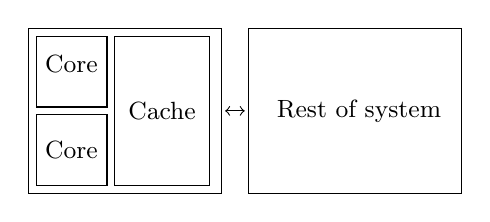
\begin{tikzpicture}
\draw (-0.5, -0.5) rectangle ++(0.9, 0.9);
\draw (-0.05, 0.05) node {\small Core};

\draw (-0.5, -1.5) rectangle ++(0.9, 0.9);
\draw (-0.05, -1.05) node {\small Core};

\draw (0.5, -1.5) rectangle ++(1.2, 1.9);
\draw (1.1, -.55) node {\small Cache};

\draw (-0.6, -1.6) rectangle ++(2.45, 2.1);

\draw (2.2, -1.6) rectangle ++(2.7, 2.1);
\draw (3.6, -0.55) node {\small Rest of system};

\draw[<->] (1.9, -0.55) -- (2.15, -0.55);
\end{tikzpicture}
\end{center}

  \begin{itemize}
    \item Each core can execute a different thread
    \item Shared memory quickly becomes the bottleneck
  \end{itemize}
\end{frame}
%%%%%%%%%%%%%%%%%%%%%%%%%%%%%%%%%%%%%%%%%%%%%%%%%%%%%%%%%%%%%%%%%%%%%%%%%%%%%%%%

%%%%%%%%%%%%%%%%%%%%%%%%%%%%%%%%%%%%%%%%%%%%%%%%%%%%%%%%%%%%%%%%%%%%%%%%%%%%%%%%
\begin{frame}
  \frametitle{Executing 2 Threads on a Single Core}

  \begin{center}
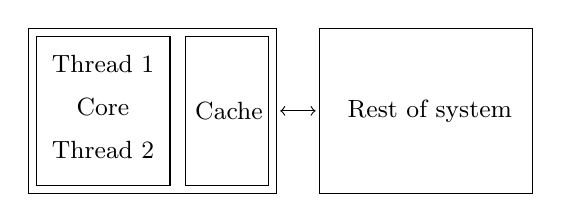
\begin{tikzpicture}
\draw (-1.4, -1.5) rectangle ++(1.7, 1.9);
\draw (-0.55, 0.05) node {\small Thread 1};
\draw (-0.55, -1.05) node {\small Thread 2};
\draw (-0.55, -0.5) node {\small Core};

\draw (0.5, -1.5) rectangle ++(1.05, 1.9);
\draw (1.05, -.55) node {\small Cache};

\draw (-1.5, -1.6) rectangle ++(3.15, 2.1);

\draw (2.2, -1.6) rectangle ++(2.7, 2.1);
\draw (3.6, -0.55) node {\small Rest of system};

\draw[<->] (1.7, -0.55) -- (2.15, -0.55);
\end{tikzpicture}
  \end{center}

  \begin{changemargin}{2.5cm}
    On a single core, must context switch between threads:
      \begin{itemize}
        \item every $N$ cycles; or
        \item wait until cache miss, or another long event
      \end{itemize}
    Resources may be unused during execution. \vfill

    Why not take advantage of this?
  \end{changemargin}
\end{frame}
%%%%%%%%%%%%%%%%%%%%%%%%%%%%%%%%%%%%%%%%%%%%%%%%%%%%%%%%%%%%%%%%%%%%%%%%%%%%%%%%

%%%%%%%%%%%%%%%%%%%%%%%%%%%%%%%%%%%%%%%%%%%%%%%%%%%%%%%%%%%%%%%%%%%%%%%%%%%%%%%%
\begin{frame}
  \frametitle{Executing M Threads on a N Cores}
\begin{center}
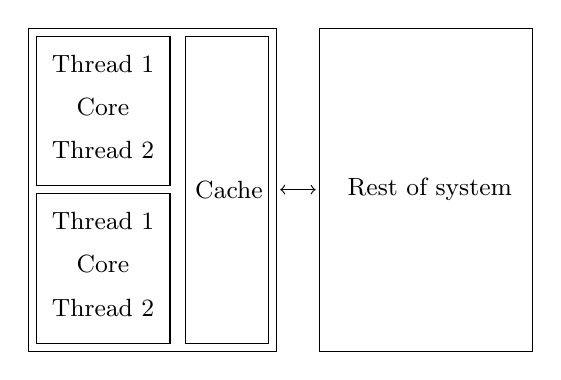
\begin{tikzpicture}

 \draw (-1.4, -1.5) rectangle +(1.7, 1.9);
 \draw (-1.4, -3.5) rectangle +(1.7, 1.9);

\foreach \y in {-2, 0}
{
 \draw (-0.55, 0.05) + (0, \y) node {\small Thread 1};
 \draw (-0.55, -1.05) + (0, \y) node {\small Thread 2};
 \draw (-0.55, -0.5) + (0, \y) node {\small Core};
}

\draw (0.5, -3.5) rectangle ++(1.05, 3.9);
\draw (1.05, -1.55) node {\small Cache};

\draw (-1.5, -3.6) rectangle ++(3.15, 4.1);

\draw (2.2, -3.6) rectangle ++(2.7, 4.1);
\draw (3.6, -1.55) node {\small Rest of system};

\draw[<->] (1.7, -1.55) -- (2.15, -1.55);
\end{tikzpicture}
\end{center}

\begin{changemargin}{2.5cm}
Here's a Chip Multithreading example. \vfill

UltraSPARC T2 has 8 cores, each of which supports 8 
threads. All of the cores share a common level 2 cache.
\end{changemargin}

\end{frame}

%%%%%%%%%%%%%%%%%%%%%%%%%%%%%%%%%%%%%%%%%%%%%%%%%%%%%%%%%%%%%%%%%%%%%%%%%%%%%%%%
\begin{frame}
  \frametitle{SMT (Simultaneous Multithreading)}

  \begin{changemargin}{2.5cm}
    Use idle CPU resources (may be calculating or waiting
          for memory) to execute another task.
    \vfill
    Cannot improve performance if shared resources are the bottleneck.
    \vfill
    Issue instructions for each thread per cycle.
    \vfill
    To the OS, it looks a lot like SMP, but gives only up to 30\% performance improvement.
    \vfill
    \item Intel implementation: Hyper-Threading.
  \end{changemargin}
\end{frame}
%%%%%%%%%%%%%%%%%%%%%%%%%%%%%%%%%%%%%%%%%%%%%%%%%%%%%%%%%%%%%%%%%%%%%%%%%%%%%%%%

%%%%%%%%%%%%%%%%%%%%%%%%%%%%%%%%%%%%%%%%%%%%%%%%%%%%%%%%%%%%%%%%%%%%%%%%%%%%%%%%
\begin{frame}
  \frametitle{Example: Non-SMP system}

\begin{center}
  \includegraphics[height=.5\textheight]{L03/ps3-small}
\end{center}

  PlayStation 3 contains a Cell processor:
  \begin{itemize}
    \item PowerPC main core (Power Processing Element, or ``PPE'')
    \item 7 Synergistic Processing Elements (``SPE''s): small vector computers.
  \end{itemize}
\end{frame}
%%%%%%%%%%%%%%%%%%%%%%%%%%%%%%%%%%%%%%%%%%%%%%%%%%%%%%%%%%%%%%%%%%%%%%%%%%%%%%%%

%%%%%%%%%%%%%%%%%%%%%%%%%%%%%%%%%%%%%%%%%%%%%%%%%%%%%%%%%%%%%%%%%%%%%%%%%%%%%%%%
\begin{frame}
  \frametitle{NUMA (Non-Uniform Memory Access)}

  \begin{changemargin}{2.5cm}
    In SMP, all CPUs have uniform (the same) access time for resources.
    \vfill
    For NUMA, CPUs can access different resources faster (resources: not just
          memory).
    \vfill
    Schedule tasks on CPUs which access resources faster.
    \vfill
    Since memory is commonly the bottleneck, each CPU has its own memory
          bank.
  \end{changemargin}
\end{frame}
%%%%%%%%%%%%%%%%%%%%%%%%%%%%%%%%%%%%%%%%%%%%%%%%%%%%%%%%%%%%%%%%%%%%%%%%%%%%%%%%

%%%%%%%%%%%%%%%%%%%%%%%%%%%%%%%%%%%%%%%%%%%%%%%%%%%%%%%%%%%%%%%%%%%%%%%%%%%%%%%%
\begin{frame}
  \frametitle{Processor Affinity}

  \begin{changemargin}{2cm}
    Each task (process/thread) can be associated with a set of processors.
    \vfill
    Useful to take advantage of existing caches (either from the last time
          the task ran or task uses the same data).
    \vfill
    Hyper-Threading is an example of complete affinity for both threads on
          the same core.
    \vfill
    Often better to use a different processor if current set busy.
  \end{changemargin}
\end{frame}
%%%%%%%%%%%%%%%%%%%%%%%%%%%%%%%%%%%%%%%%%%%%%%%%%%%%%%%%%%%%%%%%%%%%%%%%%%%%%%%%

\part{Processes vs Threads}

%%%%%%%%%%%%%%%%%%%%%%%%%%%%%%%%%%%%%%%%%%%%%%%%%%%%%%%%%%%%%%%%%%%%%%%%%%%%%%%%
\begin{frame}[fragile]
  \partpage
\end{frame}

%%%%%%%%%%%%%%%%%%%%%%%%%%%%%%%%%%%%%%%%%%%%%%%%%%%%%%%%%%%%%%%%%%%%%%%%%%%%%%%%
\begin{frame}[fragile]
  \frametitle{Background}

  \begin{changemargin}{2.5cm}
  Recall the difference between \structure{processes} and 
          \structure{threads}:
  \begin{itemize}
    \item Threads are basically light-weight processes which piggy-back on
          processes' address space.
  \end{itemize} ~\\
  Traditionally (pre-Linux 2.6) you had to use {\tt fork}~(for~processes) and {\tt clone} (for threads).
  \end{changemargin}

\end{frame}
%%%%%%%%%%%%%%%%%%%%%%%%%%%%%%%%%%%%%%%%%%%%%%%%%%%%%%%%%%%%%%%%%%%%%%%%%%%%%%%%

%%%%%%%%%%%%%%%%%%%%%%%%%%%%%%%%%%%%%%%%%%%%%%%%%%%%%%%%%%%%%%%%%%%%%%%%%%%%%%%%
\begin{frame}[fragile]
  \frametitle{History}

  \begin{changemargin}{2.5cm}
    {\tt clone} is not POSIX compliant.
    ~\\
    Developers mostly used {\tt fork} in the past, which creates a new process.
      \begin{itemize}
        \item Drawbacks?
        \item Benefits?
      \end{itemize}
  \end{changemargin}
\end{frame}
%%%%%%%%%%%%%%%%%%%%%%%%%%%%%%%%%%%%%%%%%%%%%%%%%%%%%%%%%%%%%%%%%%%%%%%%%%%%%%%%

%%%%%%%%%%%%%%%%%%%%%%%%%%%%%%%%%%%%%%%%%%%%%%%%%%%%%%%%%%%%%%%%%%%%%%%%%%%%%%%%
\begin{frame}[fragile]
  \frametitle{Benefit: {\tt fork} is Safer and More Secure Than Threads}

  \begin{changemargin}{1cm}
  \begin{enumerate}
    \item Each process has its own virtual address space:
      \begin{itemize}
        \item Memory pages are not copied, they are copy-on-write---
        \item Therefore, uses less memory than you would expect.
      \end{itemize}
    \item Buffer overruns or other security holes do not expose other~processes.
    \item If a process crashes, the others can continue.
  \end{enumerate}~\\[1em]
  {\bf Example:} In the Chrome browser, each tab is a separate process.
  \end{changemargin}
\end{frame}
%%%%%%%%%%%%%%%%%%%%%%%%%%%%%%%%%%%%%%%%%%%%%%%%%%%%%%%%%%%%%%%%%%%%%%%%%%%%%%%%

%%%%%%%%%%%%%%%%%%%%%%%%%%%%%%%%%%%%%%%%%%%%%%%%%%%%%%%%%%%%%%%%%%%%%%%%%%%%%%%%
\begin{frame}[fragile]
  \frametitle{Drawback of Processes: Threads are Easier and Faster}

  \begin{changemargin}{1cm}
  \begin{itemize}
    \item Interprocess communication (IPC) is more complicated and slower than interthread
          communication.
      \begin{itemize}
        \item Need to use operating system utilities (pipes, semaphores, shared
              memory, etc) instead of thread library (or just memory reads and writes).
      \end{itemize}
    \item Processes have much higher startup, shutdown and synchronization cost.
    \item And, \structure{Pthreads}/\structure{C++11 threads} fix issues with {\tt clone} and provide a
          uniform interface for most systems {\bf (on Assignment 1)}.
  \end{itemize}
  \end{changemargin}

\end{frame}
%%%%%%%%%%%%%%%%%%%%%%%%%%%%%%%%%%%%%%%%%%%%%%%%%%%%%%%%%%%%%%%%%%%%%%%%%%%%%%%%

%%%%%%%%%%%%%%%%%%%%%%%%%%%%%%%%%%%%%%%%%%%%%%%%%%%%%%%%%%%%%%%%%%%%%%%%%%%%%%%%
\begin{frame}[fragile]
  \frametitle{Appropriate Time to Use Processes}

  \begin{changemargin}{1cm}
  If your application is like this:
  \begin{itemize}
    \item Mostly independent tasks, with little or no communication.
    \item Task startup and shutdown costs are negligible compared to overall runtime.
    \item Want to be safer against bugs and security holes.
  \end{itemize}
  Then processes are the way to go. \\[1em]

  For performance reasons, along with ease and consistency, we'll use
  \structure{Pthreads}.
  \end{changemargin}

\end{frame}
%%%%%%%%%%%%%%%%%%%%%%%%%%%%%%%%%%%%%%%%%%%%%%%%%%%%%%%%%%%%%%%%%%%%%%%%%%%%%%%%

\end{document}
